%% abtex2-modelo-trabalho-academico.tex, v-1.7.1 laurocesar
%% Copyright 2012-2013 by abnTeX2 group at http://abntex2.googlecode.com/
%%
%% This work may be distributed and/or modified under the
%% conditions of the LaTeX Project Public License, either version 1.3
%% of this license or (at your option) any later version.
%% The latest version of this license is in
%%   http://www.latex-project.org/lppl.txt
%% and version 1.3 or later is part of all distributions of LaTeX
%% version 2005/12/01 or later.
%%aa
%% This work has the LPPL maintenance status `maintained'.
%%
%% The Current Maintainer of this work is the abnTeX2 team, led
%% by Lauro C\'{e}sar Araujo. Further information are available on
%% http://abntex2.googlecode.com/
%%
%% This work consists of the files abntex2-modelo-trabalho-academico.tex,
%% abntex2-modelo-include-comandos and abntex2-modelo-references.bib
%%

% ------------------------------------------------------------------------
% ------------------------------------------------------------------------
% abnTeX2: Modelo de Trabalho Academico (tese de doutorado, dissertacao de
% mestrado e trabalhos monograficos em geral) em conformidade com
% ABNT NBR 14724:2011: Informacao e documentacao - Trabalhos academicos -
% Apresentacao
% ------------------------------------------------------------------------
% ------------------------------------------------------------------------

\input{preambulo}

% ---- compila o \'{\i}ndice  ----
\makeindex
\makenomenclature
% ---

% ---- In\'{\i}cio do documento ----
\begin{document}
% For loading this file the following package and lines are 
% required in main latex file:
%
%   \usepackage[acronym]{glossaries}
%   \loadglsentries{acronyms}
%   \makeglossaries
%
% The entries follows are according to the line:
% \newacronym{<label>}{<abbrv>}{<full description>}

%[A]



% \newacronym{ALTO}{ALTO}{Application-Layer Traffic Optimization}
\newacronym{API}{API}{Application Programming Interface}
\newacronym{AaaS}{AaaS}{ALTO as a Service}
\newacronym[\glsshortpluralkey=ASes]{AS}{AS}{Autonomous System}
\newacronym{ASN}{ASN}{Autonomous System Number}
%[B]
\newacronym{BGP}{BGP}{Border Gateway Protocol}
\newacronym{BNG}{BNG}{Broadband Network Gateway}
%[C]
\newacronym{CDN}{CDN}{Content Delivery Network}
%[D]
\newacronym{DSL}{DSL} {Domain-specific language}
%[E]
%[F]
%[G]
%[H]
%[I]
\newacronym{IETF}{IETF}{Internet Engineering Task Force}
\newacronym{IXP}{IXP}{Internet eXchange Point}
\newacronym{ISP}{ISP}{Internet Service Provider}
%[J]
%[K]
\newacronym{KP}{KP}{Knowledge Plane}
%[L]
\newacronym{LG}{LG}{Looking Glass}
%[M]
\newacronym{MACSAD}{MACSAD}{Multi-Architecture Compiler System for Abstract Dataplanes}
%[N]
\newacronym{NFPA}{NFPA}{Network Function Performance Analyzer}
\newacronym{NFV}{NFV}{Network functions virtualization}
\newacronym{nat}{NAT}{Network Address Translation}
%[O]
\newacronym{OS}{OS}{Operating System}
\newacronym{onf}{ONF}{Open Networking Foundation}
\newacronym{odp}{ODP}{OpenDataPlane}

%[P]
\newacronym{P4}{P4}{programming protocol-independent packet processors}
%[Q]
\newacronym{QoS}{QoS}{Quality of service}
%[R]
%[S]
\newacronym{SDN}{SDN}{Software-Defined Networking}
\newacronym{SP}{SP}{Service Provider}
%[T]
%[U]
%[W]
\newacronym{WAN}{WAN}{Wide Area Network}
%[V]
\newacronym{VM}{VM}{Virtual Machine}
\newacronym{VoD}{Vod}{Video-on-Demand }
%[X]
%[Y]
%[Z]



% Retira espa\c{c}o extra obsoleto entre as frases.
\frenchspacing

% ---- ELEMENTOS PR\'{E}-TEXTUAIS ----
\pretextual

\pagenumbering{roman}

% --- Capa ---
\imprimircapa
% ---

% --- Folha de rosto (o * indica que haver\'{a} a ficha catalogr\'{a}fica) ---
\setcounter{page}{3}
\imprimirfolhaderosto*
% ---

% --- Inserir a ficha catalogr\'{a}fica ---

% Isto \'{e} um exemplo de Ficha Catalogr\'{a}fica, ou ``Dados internacionais de
% cataloga\c{c}\~{a}o-na-publica\c{c}\~{a}o''. Voc\^{e} pode utilizar este modelo como refer\^{e}ncia.
% Por\'{e}m, provavelmente a biblioteca da sua universidade lhe fornecer\'{a} um PDF
% com a ficha catalogr\'{a}fica definitiva ap\'{o}s a defesa do trabalho. Quando estiver
% com o documento, salve-o como PDF no diret\'{o}rio do seu projeto e substitua todo
% o conte\'{u}do de implementa\c{c}\~{a}o deste arquivo pelo comando abaixo:

% --- Para a vers\~{a}o final, delete as linhas abaixo e insira a linha do \includepdf
 \begin{fichacatalografica}
    \vspace*{\fill}
    \begin{center}
        \textsc{Inclua aqui o pdf com a ficha catalogr\'{a}fica fornecida pela BAE.}
    \end{center}
    \vspace*{\fill}
% --- --- ---
    %\includepdf{ficha-catalografica.pdf}
 \end{fichacatalografica}
% ---


% --- Inserir folha de aprova\c{c}\~{a}o ---

% Isto \'{e} um exemplo de Folha de aprova\c{c}\~{a}o, elemento obrigat\'{o}rio da NBR
% 14724/2011 (se\c{c}\~{a}o 4.2.1.3). Voc\^{e} pode utilizar este modelo at\'{e} a aprova\c{c}\~{a}o
% do trabalho. Ap\'{o}s isso, substitua todo o conte\'{u}do deste arquivo por uma
% imagem da p\'{a}gina assinada pela banca com o comando abaixo:

% --- Na vers\~{a}o final, exclua essas linhas e insira o \includepdf
\newpage
\vspace*{\fill}
\begin{center}
    \textsc{Inclua aqui a folha de assinaturas.}
\end{center}
\vspace*{\fill}
\newpage
% --- --- ---
%\includepdf[pagecommand={\thispagestyle{plain}}]{folha-assinaturas.pdf}	
\cleardoublepage


% ---

\begin{resumo}
    \vspace{\onelineskip}
\acrfullpl{BNG} play a crucial role in today’s networks, it hands all access network traffic (e.g., DSL traffic), provisioning of such policies like rate limiter, tunneling, and complex network management mechanisms that a \acrfullpl{ISP} needs to implement his services. These network devices are expensive, proprietary, limited and slow device upgrading, become a point of failure to deploy new features, add functionalities and correct issues on the network without disrupting the normal service operation.\\
In this work, we propose a software-based virtualized BNG device running on inexpensive commodity hardware using high-level language for programming protocol-independent packet processors over a  Multi-Architecture Compiler System to remove some of these barriers to innovation.\\


    \noindent\textbf{Keywords}: Computer Networks; Software Defined Networking; OpenFlow; Future Internet.

    % \vspace{\onepageskip}
    % \vspace{\onelineskip}
    \pagebreak

    \begin{otherlanguage*}{portuguese}
    \begin{center}{\ABNTEXchapterfont\huge Resumo}\end{center}
    
Adicionar resumo em portugues...
%         \textit{OpenFlow} é a mais proeminente tecnologia para a implementaç\~{a}o de Redes Definidas por Software (RDS). Projetada como uma interface de controle entre switches e controladores, o protocolo pode ser visto como um conjunto de instruç\~{o}es para programar a l\'{o}gica de encaminhamento em comutadores da rede. A primeira vers\~{a}o do \textit{OpenFlow} atraiu a atenção de pesquisadores da ind\'{u}stria e universidades interessados nos potenciais benef\'{i}cios prometidos por RDS. R\'{a}pidamente surgiram ferramentas para experimentação em \textit{OpenFlow} 1.0, incluindo comutadores, controladores e software para testes e emulaç\~{a}o. Ap\'{o}s o in\'{i}cio da padronizaç\~{a}o do protocolo pela \textit{OpenNetworkFoundation}, o protocolo OpenFlow evoluiu rapidamente dando origem \`{a} novas especificaç\~{o}es. As novas funcionalidades aumentaram as possibilidades de experimentos, gerando entusiasmo. Porém, o desenvolvimento das ferramentas de experimentaç\~{a}o n\~{a}o acompanharam o mesmo r\'{i}tmo do protocolo. Para preencher essa lacuna, esse projeto desenvolveu um comutador em \textit{software} com suporte a \textit{OpenFlow} 1.3. Guiado pelo objetivo de ser simples e básicos requerimentos de performance, a proposta da ferramenta \'{e} ser uma opç\~{a}o, f\'{a}cil e funcional para desenvolvedores de aplicaç\~{o}es RDS  buscando utilizar as novas funcionalidades do \textit{OpenFlow} 1.3. Em suma, o \textit{software} desenvolvido nesse projeto foi o primeiro comutador \textit{OpenFlow} 1.3 do mundo. Lançado como projeto de c\'{o}digo aberto, possibilitou a pesquisadores de todo o mundo a prototipagem e demonstraç\~{a}o de soluç\~{o}es n\~{a}o poss\'{i}veis anteriormente.

    \vspace{\onelineskip}

    \noindent\textbf{Palavras-chaves}: Redes de Computadores, Software Defined Networking, OpenFlow, Internet do Futuro. 

    \end{otherlanguage*}
\end{resumo}

% --- RESUMOS (em ingl\^{e}s ---
% \begin{resumo}

%     \begin{otherlanguage*}{english}   
%     \lipsum[2]

%     \vspace{\onelineskip}

%     \noindent\textbf{Keywords}: Computer Networks; Software Defined Network; OpenFlow; Internet of Future.

%     \end{otherlanguage*}
% \end{resumo}
% ---

% --- inserir o sumario ---
\pdfbookmark[0]{\contentsname}{toc}
\tableofcontents*
\cleardoublepage
% ---

% --- Dedicat\'{o}ria ---
\begin{dedicatoria}
    \vspace*{\fill}
    \centering
    \noindent
    \textit{When a goal is reached, it is necessary to think and value those things that led us to reach it; the walked path and the learned lessons.  I would like to dedicate this work all the people who gave me their prayers, words of encouragement but also his wisdom, love and support; this goal has been possible thanks all of you.  I am sure that in any place God will allow us to meet  people like you to keep growing in both personal and professionally.} 
    
    \vspace*{\fill}
\end{dedicatoria}
% ---

% --- Agradecimentos ---
\begin{agradecimentos}
   
My thanks to my parents, whoever has motivated me to go further and give me the best example of dedication. \\
I am grateful for my family, for his support in the distance and send me his best wishes and prays.

Christian Esteve Rothenberg, my supervisor, and friend.
Many thanks to INTRIG group for bringing me support many times and even for its friendship outside of the university.

Ericsson Innovation Center Brazil, for sponsoring this work, and Ericsson Traffic Lab in Hungary, for technical support.

% Finally, my sincerely acknowledgments to people who collaborated with code, bug reports or suggestions.



    
    
\end{agradecimentos}
% ---

% --- Ep\'{\i}grafe  ---
\begin{epigrafe}
    \vspace*{\fill}
	\begin{flushright}
		\textit{``The true sign of intelligence is not knowledge but imagination''\\
		Albert Einstein}
	\end{flushright}
\end{epigrafe}
% ---


% --- inserir lista de ilustra\c{c}\~{o}es ---
\pdfbookmark[0]{\listfigurename}{lof}
\listoffigures*
\cleardoublepage
% ---

% --- inserir lista de tabelas ---
\pdfbookmark[0]{\listtablename}{lot}
\listoftables*
\cleardoublepage
% ---

% --- inserir lista de Acronimos e Abrevia\c{c}\~{o}es ---
\renewcommand{\nomname}{Acronyms and Abbreviations List}
\pdfbookmark[0]{\nomname}{las}
\nomenclature{ARP}{Address Resolution Protocol}
\nomenclature{API}{Application Programming Interface}
\nomenclature{ASIC}{Application Specific Integrated Circuit}
\nomenclature{BNG}{Broadband Network Gateway}
\nomenclature{CAM}{Content Addressable Memory}
\nomenclature{CRC}{Cyclic Redundancy Check}
\nomenclature{DSCP}{Differentiated Services Code Point}
\nomenclature{Kbps}{Kilobits per second}
\nomenclature{Kpps}{Kilo packets per second}
\nomenclature{ICMP}{Internet Control Message Protocol }
\nomenclature{IP}{Internet Protocol}
\nomenclature{IPv6}{Internet Protocol Version 6}
\nomenclature{JSON}{JavaScript Object Notation}
\nomenclature{MAC}{Media Access Control}
\nomenclature{Mbps}{Megabits per second}


\nomenclature{ONF}{Open Network Foundation}
\nomenclature{OVS}{Open vSwitch}
\nomenclature{QoS}{Quality of Service}
\nomenclature{RAM}{Random Access Memory}
\nomenclature{SDN}{Software Defined Networking} 
\nomenclature{TCP}{Transmission Control Protocol}
\nomenclature{TTL}{Time to live}

\printnomenclature



\cleardoublepage
% ---

\pagenumbering{arabic}

% ---- ELEMENTOS TEXTUAIS ----
\textual

% ---- Introdu\c{c}\~{a}o ----
\chapter{Introduction}
\label{cap:intro}
The advent of new services like \acrfull{VoD}, video conference, Virtual Private Network (VPN) and cloud-based new services, has increased the demand for access to broadband services \cite{improv}.  In addition, many further access technologies such as xDSL, optical access and wireless technologies such as WiMAX and LTE require rapid deployment of services and devices guaranteeing performance in Internet Services provider (ISP) networks.\\
In an Internet service provider (ISP) network the Broadband Network Gateway (BNG) has the function of managing all access network traffic (e.g., DSL traffic) and other critical functions like to allow access and authentication for thousands of subscribers, monitoring, establishing sessions, tunnels and controls the user line rate.  The fact that all sessions tunnels (e.g.., PPPoE, GRE) are terminated at the BNG means that is aggregated in a single point causing poor performance and quality of service.
Therefore is no surprise that this device becomes expensive and hardware proprietary boxes, often the operator pay for some functionality that won’t be used and the hardware boxes upgrade require a long wait until the next version available.\\
In recent years, in order to resolve this problem to turn this rigid hardware device into a software-based network and reduce time to market of new services and those functionalities have been decomposed and dynamically instantiated at different points of the network. This concept is following the trend of \acrfull{SDN}  and \acrfull{NFV} that turn some network functionalities into virtualized software processing running on a server (e.g., off-the-rack x86 servers), switches or even cloud computing infrastructure \cite{nfv}.\\
Our approach to create an fully open and programmable BNG data plane is using a high-level language for \acrfull{P4}, this is a \acrfull{DSL} with a number of functions optimized around network data forwarding.\\
Such a DSL can support customizing the forwarding behavior of the switch and may also be ported to other hardware or software switches that support the same language.
In this work, we present an approach to implementing a BNG software switch implementation, and it is built on top of the MACSAD Switch target and P4 language that can provide dynamic and flexibility to the service provider to optimize the traffic on the network.\\
We discuss the architecture and protocols to deploy and concepts around the BNG software switch.\\
The rest of this document is structured as follows: Section II provides the background and related work.  Section III The problem statement and objectives, Section IV and Introduces the proposed design and some results, Section V Working plan and Execution schedule.

\section{Objectives}
\label{sec:sec02}
To address the identified issues, the main objective of this work is to design, implement and evaluate the \acrshort{BNG} software switch in a Multi-Architecture Compiler System for Abstract Dataplanes (MACSAD). To this end, the following specific objectives are proposed: 

For each of the issues mentioned in section ~\ref{sec:ProblemStatement}, we have some specific objectives in order to take action to those problems:

\begin{itemize}

\item Designing the architecture and functional implementation of a BNG software switch.  Adding the data plane functionalities with the latest version of P4 lang and compiling our BNG p4 program in an emulation environment in order to test our P4 implementation.

\item Defining and implementing P4$_{16}$ support for MACSAD.  The MACSAD core works with C code in order to compile and run the software switch at execution time over a commodity server. According to the above, we need to implement the HLIR16 project and his dependencies such as P4C compiler to create an intermediate representation that brings data structure used internally in the MACSAD core to translate P4 into C.

\item Integrating the BNG implementation generated with MACSAD to support the Traffic Manager ODP API.  It adds QoS support to the BNG software switch.  On the other hand,  the controller has to interact either with MACSAD to manage table actions management as with the Traffic Manager block hence; this interface will be added as well. 

\item Performance evaluation with NFPA tool. Configuring a real network testing environment, software and hardware such as the described in section 5 in order to evaluate the packet processing performance with some specific use cases recommended in \cite{Nemeth}:
\begin{itemize}
 \item Port Forwarding/L2 forwarding
 \item L2 forwarding
 \item GRE Encap/Decap
\end{itemize}
Evaluating with unidirectional traffic and Small (64B) to large (1518B) packet sizes and with fixed destination and source MAC addresses, IP addresses and ports.


\end{itemize}




\section{Text Structure}
\label{sec:sec03}

In this Introduction we explained the motivational aspects that justify this work. Also, we give a clear explanation for the objectives of this project. 

In Chapter~\ref{cap:cap02} we present a Literature Review. Related  to\gls{P4} language, \gls{odp} SDK and MACSAD framework architecture are described in the context of our implementation requisites.

% are discussed from the point of view of our implementation requisites. 

In Chapter~\ref{cap:cap03} we take a look at the architecture of the BNG software switch which we explain all the modules an his relationship between. Furthermore, we describe the tables associated to BNG dataplane.

In Chapter~\ref{cap:cap04} we explain the BNG functionalities and features in detail.

In Chapter~\ref{cap:cap05} we show the performance results and compare with related work.

Finally, in Chapter~\ref{cap:conclusion} we highlight the results, issues in the implementation process and future work.

% we give our conclusion remarks. This chapter highlights results, presents known use cases and discusses possible improvements in future works. 



% ---- Cap\'{\i}tulos ----
\chapter{Literature Review}
\label{cap:cap02}
 This section defines three main concepts in our research work: \acrshort{BNG} Protocol, another is the \acrshort{P4} language, the third MACSAD compiler and finally an ODP framework description.

\subsection{Broadband Network Gateway}

 The first generation network based on centralizes BRAS routers was driven for the customer demand for High-speed Internet (HSI) the second generation Ethernet-based Broadband Network Gateway (BNG) routers was driven by subscriber demand for a linear TV service (content broadcast at specific times, e.g., Netflix) delivered in conjunction with voice and HSI services \cite{Alcatel}.\\
 The Customer Premise Equipment (CPE) represents the triple play communications devices: Telephone (Voice), PC (Internet), Set-top box (TV) however all these devices are connected to a Home Gateway (HG) that brings the interface with the network through any access technology like Digital Subscriber Line (DSL).\\
 One or more HG can be connected to a single DSLAM that sends the traffic to the BNG device and it route in a core IP network and the edge routers to provide connectivity to the Internet (See Figure \ref{fig:arch}).\\
 \begin{figure}[!h]
 	\centering
 	\includegraphics[width=0.8\linewidth]{figures/bng_architect.png}
 	\caption{Access Network Provider Model.}
 	\label{fig:arch}
\end{figure}
The network operator provides connectivity, authentication, applications and service network  policies to his users, therefore, these procedures involve the premise of session establishment using access communication protocols which are managed in the BNG, the most common protocols to establish session are:
\begin{itemize}
\item The PPP over Ethernet (PPPoE): Use the point-to-point (PPP) protocol.
\item The IP over Ethernet (IPoE): Use IP protocol that runs between CPE and BNG.
\item Generic Routing Encapsulation (GRE V2), encapsulation protocol brings virtual  Point-to-Point connections through IP network.
\end{itemize}
In our implementation, the packet sent or received by the HW are encapsulated with GRE headers, creating a point-to-point link with the BNG, but is just one of the options for packets encapsulation. \\
Since the BNG centralizes all the functions simplify the management functions like:
\begin{itemize}
\item Session management and header cap/decapsulation.
\item Interface to Authorization, Authentication and accounting services.
\item ARP proxy to manage the requests from the network interface on the BNG side.
\item Network Address translation to route the packets towards the operator’s core Network.
\item Interface to assignment queues and line rate to subscribers.
\end{itemize}
On the other hand, all these tasks make the structure of network rigid and become difficult to support the protocols and architectures in the current ISP.  In \cite{Rethinking} we found some similar approach to virtualize a Broadband Remote Access Server (BRAS) based on Click OS, a tiny Xen virtual machine designed specifically for network processing it can achieve line rate of 10Gbps and it composes of netmap and VALE as the packet I/O framework.
Our architecture approach goes with the same trend of network function virtualization using Macsad framework that compiles P4 code to bring more flexibility to the data plane and adding support for Hardware Abstraction Layer (HAL).\\
In the next session, we will describe our architecture design to be rapidly reconfigured using a “programming protocol-independent packet processors” (P4) and MACSAD to generate the datapath Logic codes.


% %%%%%%%%%%%%%%%%%%%%% subSection 2 P4 %%%%%%%%%%%%%%%%%%%%%%%%%%%%%%%%%%%
\subsection{Programming Protocol-Independent Packet Processors (P4)}
\begin{figure}[!h]
	\centering
	\includegraphics[width=0.7\linewidth]{figures/p4_dp.png}
	\caption{P4 Abstract Forwarding Model. Source: Adapted from \cite{P4}.}
	\label{fig:p4_dp}
\end{figure}
P4 is a high-level language for programming protocol-independent packet processors that define how the pipeline of a network forwarding device should process the packets using the abstract forwarding model (See figure \ref{fig:p4_dp}). P4 define the header structures and use the parser to extracts the header fields. The pipeline is defined through a series of match-action tables, which execute one or more actions like packet forwarding, drop and so on.  This tables can be changed and accessed at "runtime" through a controller software to add, remove and modify table entries and finally, de-parser writes the header fields back before sending the packets to the output port. The three main advantages of P4 are:

\begin{enumerate}
\item Reconfigurability in the field: Programmers should be able to change the way how the switch process the packets once that was deployed. 
\item Protocol independence: Capability to deploy any protocol in a switch.  
\item Target independence: To describe packet-processing functionality independent of the hardware where it has been deployed \cite{P4}.
\end{enumerate}

% %%%%%%%%%%%%%%%%%%%%% subSection 2 MACSAD %%%%%%%%%%%%%%%%%%%%%%%%%%%%%%
\subsection{Multi-Architecture Compiler System for Abstract Dataplanes (MACSAD)} 
\label{sec:Macsad}
This tool brings an environment to compile and deploy switch for L2/L3 applications automatically generating the datapath code for heterogeneous targets over 10Gbps network interfaces setup \cite{Patra}.\\
The MACSAD architecture is designed around the following three modules: (See the figure 2a) \\ \\
\begin{figure*}[!ht]
	\centering
	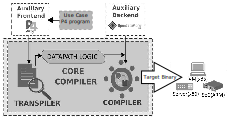
\includegraphics[width=0.85\linewidth]{figures/macsad_arch.png}
	\caption{Macsad architecture. Source:\cite{Patra}}
	\label{fig:mac_arch}
\end{figure*}

\textbf{- Auxiliary Frontend:} The P4 code is the MACSAD input that will be converted to an IR representation using the  p4-hlir framework that supports different Domain Specific Language (DSL) to generate a High-Level Intermediate Representation (HLIR) to be used in the Macsad core compiler.\\
\textbf{- Auxiliary Backend:} this module provides a common SDK for the Compiler incorporating the ODP APIs 
%  \cite{odp} 
 auto-generating support for different platforms with ODP supporting various control protocols like Switch Abstraction Interface (SAI), OpenFlow (OF), and other useful events for buffer like queueing, scheduling, etc.\\
\textbf{- Core Compiler:} Composed of a Transpiler and a Compiler submodule (see the figure \ref{fig:mac_arch}b), transforms the IR generated by the frontend into the target imaged in association with the auxiliary backend.\\
The transpiler takes the HLIR input and auto-generates the Datapath Logic codes. Some critical decision is taken in this sub-module like to optimize the ’Dead Code Elimination’ by identifying reachability in a graph, decides the type of look-up mechanism to be used, and size and type of tables to be created by. 
The Macsad compiler creates a set of libraries in 'C' codes for the desired target (x86, x86+DPDK, ARM-SoC).\\
The BNG P4 code will be added to the system as an input to create the BNG router. Also, Macsad tool brings the generation of high-level ODP APIs to deliver platform abstraction with high performance and hardware-acceleration options.



\subsection{Open Data Plane (ODP)}
Open Data Plane project provides an application programming environment for data plane applications with high performance and portable across a lot of HW platform.
The aim of ODP is separate application design from the functional implementation of that design, this because historically it requires that data plane application must be redesigned on changes in network speed and capacity because the applications need to be very integrated with specialized hardware to achieve acceptable performance levels.
ODP relies on the Linux kernel itself; it defines some ODP API set to rapid porting ODP application to any platform (See Figure \ref{fig:sys_arch}), it can define functions and limits like a number of queues or used cores processor.\\
% %%% -----------
\begin{figure*}[!ht]
	\centering
	\includegraphics[width=0.6\linewidth]
     {figures/odp-overview.png}
% 	\caption{ODP system architecture. Source:\cite{opd_spec}}
 	\caption{ODP system architecture. Source:....}
	\label{fig:sys_arch}
\end{figure*}
ODP applications can run in parallel with full Linux user processes that implement control and management functions since that these typically do not have critical performance and latency requirements. In that sent, this tool calls the Software Development Kit (SDK) and optimize the features and functionalities for the particular hardware platform (SoC or Server).
The ODP APIs is written in the C programing language and are optimized to control related SoC resources such as:
\begin{itemize}
\item CPUs (or hardware threads) 
\item Main memory
\item Huge page mappings (how many, what sizes) 
\item Physical and virtual ports/interfaces 
\item Packet classification rules 
\item Scheduler (core groups, algorithms, ordering) 
\item Hardware queues 
\item Output traffic management 
\item hardware Quality of Service (QoS) support. 

\end{itemize}

\subsection{NFPA}

\chapter{Architecture}
\label{cap:cap03}

The Architecture overview is shown in Figure \ref{fig:bng_arch}. We have main tree processes: (i) Creation of BNG data plane, (ii) Macsad P4\_16 support and (iii) Integration with OPD APIs. Finally, this network virtualized device can be used in a commodity server such as executable program.

\begin{figure*}[ht]
	\centering
	\includegraphics[width=0.7\linewidth] {figures/bng_arch_0.png}
	\caption{BNG software architecture.}
	\label{fig:bng_arch}
\end{figure*}


\begin{enumerate}
\item Create a P4 program in order to set the data plane functionalities of the BNG device (BNG data plane).   
\item Adds support the the current MACSAD implementation in order to compile the last version of P4 (P4\_16). 	
\item Integration of the BNG compiled and generated version by MACSAD with the ODP APIs, to add others features like Traffic management, Scheduling, and Rate limiter.

\end{enumerate}

Details of processes are explained in the next sections. It is important to highlight that the first process was completed, the second and third are currently in progress and the latter process is included as a scheduled task in Working Plan and Execution Schedule chapter.


\subsection{Creation of BNG data plane }
\label{ss:dataplane}
\begin{figure*}[ht]
	\centering
	\includegraphics[width=0.7\linewidth] {figures/bng_pipe.png}
	\caption{BNG data plane.}
	\label{fig:bng_pipe}
\end{figure*}

To support the workload multiples lookup tables are supported either Upload link (UL) and Download Link (DL): a table to store MAC address, a table of CPE based on their IP address routing table, encap/decap GRE, both tables to block any port or IP using a Firewall for UL and DL, both table to Network Address translation (NAT) for UL and DL, the table to limiter the user rate either UL and DL. They are briefly described below.

\subsubsection{L2 mac table}
When the L2 packet is coming to the BNG switch, it uses MAC learning. Hence, when an ARP packet is received from the CPE, an entry is created (or updated) in a MAC address table swap the source and destination MAC address in the Ethernet header.\\
Ethernet is the protocol used in the Transport layer.  Therefore, the packet header fields are read and rewrite with the new fields in this table in order to forward the packet out by the appropriate port.

\subsubsection{Nat table}
Basic full-connect NAT for TCP traffic (over IPv4) do both main functions:
Translates IPv4 addresses and TCP port numbers of request packets originating from a client on a private network (iAddr: iPort) is mapped to an external address (eAddr: ePort), any packets from iAddr: iPort is sent through eAddr: ePort, the packets that his header fields matching in NAT table are processed in order to rewrite the new header and the packet is forwarded appropriately otherwise when a TCP packet is received on the external interface, for which there is no mapping, the packet is dropped.

\subsubsection{GRE tables}
The BNG will be able the forward based on the contents of a custom encapsulation header as well as perform normal IP forwarding if the encapsulation header does not exist in the packet.
Our BNG is enabled to create point-to-point tunnel mechanism in the intern network to encapsulate the packets with standard GRE packet header structure, as defined by RFC 2784 and RFC 2890 and save the user ID in order to establish the user session.\\
The BNG de-encapsulate the packets originated from CPE to an external address as well as the reverse process when the packet incoming from an external network.  The GRE table encap has the outer IP address header field in order add it as new IPv4 header and the GRE header fields in order to enable the new packet.

\subsubsection{IPV4 table}
The routing table stores the next hop based on the IP address. It’s based on the LPM (longest prefix match) implementation. Another table stores information related to the next hop (IP address, port index, etc.).
With IPv4 forwarding, the switch must perform the following actions for every packet: (i) update the source and destination MAC addresses, (ii) decrement the time-to-live (TTL) in the IP header, and (iii) forward the packet out the appropriate port.
Our BNG device will populate with static rules using a basic controller.  Each rule will map an IP address to the MAC address and output port for the next hop.

\subsubsection{Parser/Deparser}
Our parser will detect the different headers used in the BNG device. It extracts headers from the packet at the current offset into per-packet header instances and marks those instances valid, updating the Parsed Representation of the packet. The parser then indicates as valid byte the correct header and makes a state transition to the next header.
The de-parser reverses the process of parsing that emits headers in the proper order. Only headers which are valid are serialized, in our case, the output packet is serialized with the same protocols of the input parser block.

\subsubsection{Rate limiter}
Some research works [i.e \cite{Rodrigues},\cite{Popa},\cite{Ballani}]  based on end host-based rate enforcement for fair and guaranteed bandwidth allocation  in a  multi-tenant datacenter. 
A datacenter requires a large number of rate limiters, far of the capacity of commodity NICs (e.g., Intel’s 82599 10G NIC supports up to 128 rate limiters). Software rate limiters in host network stacks can scale, but this approach implies high CPU overheads hinder support for high-speed links \cite{Radhakrishnan_2014}
We implemented a basic Rate limiter in P4 code without slow down performance for every packet to inspect such as defined in RFC 2698 (A Two Rate Three Color Marker - IETF) standard; these describe traffic policing elements like a meter and a dropper.  The meter measures the traffic and determines whether or not it exceeds the rate limit, in case that it exceeds the limit the packets could be dropped.


\subsection{Macsad P4$_{16}$ support}
Macsad is in charge of converting our BNG P4 program into C code, specifically, it brings support to the version P4$_{14}$ (v1.0/v1.1). However, since may of 2017 has been launched the new version P4$_{16}$ (v1.0) that compared with the early version doing larges changes regarding syntax and semantics of the language.
The new P4$_{16}$ specification\footnote{https://p4lang.github.io/p4-spec/docs/P4-16-v1.0.0-spec.pdf} shows in figure \ref{fig:p4_evol} how this has been transformed from a complex language (more than 70 keywords) into a more compact language (less than 40 keywords) accompanied by a library of fundamental constructs that are needed for writing most of the P4 programs.

\begin{figure*}[ht]
	\centering
	\includegraphics[width=0.7\linewidth] {figures/p4_evol.png}
	\caption{Evolution of the language between versions P4$_{14}$ (v 1.0 and 1.1) and P4$_{16}$.  
%  Source \cite{p4_evolu}}
    }
 	\label{fig:p4_evol}
 \end{figure*}

As we can see the section 
% \ref{sec:Macsad},
in the Frontend layer, MACSAD is using p4-hlir project which translates P4 programs into High-Level Intermediate Representation (HLIR) that creates a suitable P4 program representation (See figure \ref{fig:mac_arch}b), that can be consumed by multiple back-ends, in our case, MACSAD will be used this tool in “Transpiler module”, where is access the different P4 top-level objects using these Python ordered dictionary such as p4\_parser, p4\_tables, p4\_actions, p4\_headers and so on.\\
Therefore, our approach for MACSAD update to the new version is using HLIR16 project 
% \cite{hlir16}
that create a convenient Python representation from a JSON file compiled in P4C compiler from a .p4 source file. 


\subsection{Integration with OPD API's}

In order to apply some quality-of-services options for the ISP users, exist some mechanism for achieving these kinds of traffic-management goals in a shared network is through queuing and scheduling. This below features working together, deciding what packets get sent and when; thus scheduling is in charge of sending someone else’s packets right now or delaying packets that are arriving too fast.
In the following subsection, we will take a look at so-called Weighted fair queuing (WFQ) that provides a straightforward strategy for dividing bandwidth among multiple senders according to preset percentages.


\subsubsection{Weighted fair queuing (WFQ)} 

% \begin{figure}[ht]
% \centering
%   \subfigure[]
%   {
%     \raisebox{10mm}
%     {
%       \includegraphics[scale=0.5] 
%       {figures/wfq_diag.pdf}
%       \label{fig:wfq_diag}
%     }
%   }
%   \subfigure[]
%   {
%   	\includegraphics[scale=0.2]
%     {figures/tm_node.png}
%     \label{fig:tm_Node}
%   }
% \caption{(a)Weighted Fair Queuing priority.  Source (b) Traffic Manager Node.  Source  }
% \end{figure}


% \caption{(a)Weighted Fair Queuing priority.  Source \cite{anintro} (b) Traffic Manager Node.  Source \cite{opd_spec} }
% \end{figure}



This is a data packet scheduling algorithm based on both Fair Queueing (FQ) and the generalized processor sharing policy (GPS), where instead of giving each class an equal share, we assign each class a different percentage. For example, If all four input classes A,B,C,D are active, then each gets 25\% of the total bandwidth (see figure \ref{fig:wfq_diag}), just as for a flat four-input-class fair queuing structure. However, when only A, B and C are active, and D is idle.  A, B and C each get 33\%, hence it lets to allocate bandwidth according to administratively determined percentages.\\ 
ODP provides a suite of APIs that control traffic shaping and Quality of Service (QoS). Tx processing using Traffic manager and RX processing involves the use of Scheduler, both processes are described around in the next subsections.


\subsubsection{Scheduled RX Processing}
Scheduled RX processing is performed via the Scheduler and is requested when a PktIO is opened with an in\_mode of ODP\_PKTIN\_MODE\_SCHED.
In a basic use, it associates the PktIO input event queues created by odp\_pktin\_queue\_config() with the scheduler. The hash function could be employed to distribute input packets among multiple input queues and instead of these being plain queues they have scheduled queues and have associated scheduling attributes like the priority, scheduler group, and synchronization mode (parallel, atomic, ordered). 



% \subsubsection{Scheduled RX Processing}
% Scheduled RX processing is performed via the Scheduler and is requested when a PktIO is opened with an in\_mode of ODP\_PKTIN\_MODE\_SCHED.
% In a basic use, it associates the PktIO input event queues created by odp\_pktin\_queue\_config() with the scheduler. The hash function could be employed to distribute input packets among multiple input queues and instead of these being plain queues they have scheduled queues and have associated scheduling attributes like the priority, scheduler group, and synchronization mode (parallel, atomic, ordered). 
 \begin{figure}[ht]
 	\centering
 	\includegraphics[width=0.55\linewidth] 
     {figures/pktin_sched_recv.png}
  	\caption{PktIO SCHED Mode Receive Processing.  Source} 
% \cite{opd_spec}}
 	\label{fig:pktin_sched}
 \end{figure}

Inbound packets are classified and put on queues associated with their target class of service which are themselves scheduled to threads (see figure \ref{fig:pktin_sched}). 

\subsubsection{Scheduled TX Processing}

Scheduled TX processing is performed via the ODP Traffic Manager and is requested when a PktIO is opened with an out\_mode of ODP\_PKTOUT\_MODE\_TM. 
The ODP Traffic Manager accepts packets from input queues and applies strict priority scheduling such as weighted fair queueing scheduling and bandwidth controls to decide which input packet should be chosen as the next output packet and when this output packet can be sent onwards.\\
Weighted Fair Queuing (WFQ) is used for priority assign from multiple input packets with the same priority. Each input can be assigned a weight in the range MIN\_WFQ\_WEIGHT to MAX\_WFQ\_WEIGHT (nominally 1..255) that affects the way the algorithm chooses the next packet. If all of the weights are equal AND all of the input packets are the same length then the algorithm is equivalent to a round-robin scheduling.\\

A TM system is composed of Tm\_nodes are "entity"/object. It lets interconnect, and interplay of a multi-level "tree" of tm\_nodes can allow the user to specify some very sophisticated behaviors. Each tm\_node can contain a set of WFQ scheduler (see figure \ref{fig:tm_Node}).  Each node contains a set of "fan-in" connections to preceding tm\_queues or tm\_nodes.

\chapter{Development}
\label{cap:cap04}

This chapter covers the software switch development. In section \ref{softfeatures}, we give details about the implementation of the most important BNG features.

\section{Software switch implementation}
\label{softfeatures}

In this section we discuss how we implemented the BNG software switch adding several changes to the base switch - using C \footnote{In this chapter there will be two common words: struct and structure. While struct is a P4 language keyword and structure is a more generic word for a collection of data variables, both will be used to denote a C struct.}, the switch native programming language, and C++ - in order to support all features and keep it as simple as possible.

\subsection{soporte a primitivas}

\begin{itemize}

\item add header

\item remove header

\item drop
\end{itemize}


 
\chapter{Evaluation}
\label{cap:cap05}

In this chapter we evaluate our work in terms of the requisites presented on section \ref{sec:sec02}. The first section shows in numbers how many features are covered by the software switch. Subsequently, in the next section, we present the results of performance benchmarks tests. The last section of the chapter is a qualitative evaluation about the code's ease to change. We demonstrate the code portability, highlighting the port of the software switch to another processor architecture in a different operating system.      

The software switch evaluated version dates from the last commit pushed to GitHub. The box below shows the dates and last code changes description.

\begin{framed}

\begin{itemize}
\item \textbf{commit} cb740bd2565ac7e5d61ebe30ee75160a5452a033
\item   \textbf{Commit:}     Eder Leão Fernandes <ederleaofernandes@gmail.com> 
\item \textbf{CommitDate:} Mon Feb 23 18:42:49 2015 -0300 
\end{itemize}
     
    Add flags member to ofp_flow_stats.
    
    Fix missing flags field in the response of a flow stats request.
\end{framed}

\section{Feature Completeness}
\label{sec:FeatureComplete}
Evaluating the proper operation of the OpenFlow switch features is not a trivial task. This is caused by the multiple and rich configurations allowed by the specification. For example, testing all flow match fields combinations would require creation of a large number of flows and packets, making manual tests very time consuming. For this reason, automatic test frameworks, discussed on section \ref{sec:testemulation}, are the best options to test the switch functionality in order to evaluate feature completeness.    

OFTest and Ryu Certification are the two test frameworks used for the switch validation. As mentioned in chapter \ref{CodeMaintenance}, both are important tools for the software switch development. While Ryu certification has a strong focus on validation of the Datapath, OFTest offers a nice set of test cases for control and data plane message exchange. In the next sections we present a resume of the results obtained.  


\subsection{OFTest results}

Testing in OFTest is simple as it provides scripts in Python to run the switch and the test cases. Each test case starts a controller which connects with a running switch, executes the test instructions and checks the switch answers. 

Some messages from controller to switch, like a \textit{flow stats} request, and symmetric messages demand an answer from the switch. Thus, the main purpose of the framework usage with the software switch is for message handling validation. Although OFTest has capabilities to evaluate the pipeline processing - for instance, checking if a packet was correctly forwarded by a flow - we found in Ryu a more comprehensive test set for this task. 

Table \ref{tab:oftestbasic} shows test results for basic OpenFlow messages. The major type of messages of the test set are messages to query information about the state of manifold switch elements, such as \textit{GroupFeatureStats} and \textit{MeterStats}. Also, there are some configuration messages, like the \textit{PortConfigMod}. In all tests the switch returned the right answer for the control plane.


\begin{table}[h]
\centering
\caption{Basic OpenFlow messages}
\label{tab:oftestbasic}
\begin{tabular}{|l|l|l|l|l|}
\cline{1-2} \cline{4-5}
\multicolumn{1}{|c|}{\textbf{Message}} & \textbf{Result} &  & \textbf{Message}   & \textbf{Result} \\ \cline{1-2} \cline{4-5} 
AggregateStats                         & ok              &  & GroupFeaturesStats & ok              \\ \cline{1-2} \cline{4-5} 
AsyncConfigGet                         & ok              &  & GroupStats         & ok              \\ \cline{1-2} \cline{4-5} 
DescStats                              & ok              &  & MeterConfigStats   & ok              \\ \cline{1-2} \cline{4-5} 
Echo                                   & ok              &  & MeterFeaturesStats & ok              \\ \cline{1-2} \cline{4-5} 
EchoWithData                           & ok              &  & MeterStats         & ok              \\ \cline{1-2} \cline{4-5} 
FeaturesRequest                        & ok              &  & QueueStats         & ok              \\ \cline{1-2} \cline{4-5} 
FlowStats                              & ok              &  & PortConfigMod      & ok              \\ \cline{1-2} \cline{4-5} 
FlowRemoveAll                          & ok              &  & PortDescStats      & ok              \\ \cline{1-2} \cline{4-5} 
GroupDescStats                         & ok              &  & TableStats         & ok              \\ \cline{1-2} \cline{4-5} 
\end{tabular}
\end{table}

Controller roles test results are shown in table \ref{tab:oftestrole}. These tests check if the software switch changes correctly controller roles, and if the respective permission police is respected. As in the previous message tests, all role tests were successful.    

\begin{table}[h]
\centering
\caption{Role request message results}
\label{tab:oftestrole}
\begin{tabular}{|l|l|}
\hline
\textbf{Role Request Tests} & \textbf{Results} \\ \hline
RoleRequestEqualToSlave     & ok               \\ \hline
RoleRequestSlaveToMaster    & ok               \\ \hline
RolePermissions             & ok               \\ \hline
RoleRequestEqualToMaster    & ok               \\ \hline
RoleRequestNochange         & ok               \\ \hline
SlaveNoPacketIn             & ok               \\ \hline
\end{tabular}
\end{table}

\subsection{Ryu Certification results}

The Ryu Certification tests are divided into five categories: Action, Set-Field, Match, Group and Meter. The test sets of each category are very comprehensive, with tests for different packet types.

Table \ref{tab:ryuresults} is a resume of test results - the complete list of test cases can be found on Annex \ref{annex:ryucert} - for this work compared to the other three switches presented on chapter \ref{cap:cap02}. White cells give the number of tests passed, while grey cells show the number of test cases that returned an error. Tests are divided by each category, with the last two columns giving the total sum of working and non working features. The first row presents the results for this work. \footnote{ofsoftswitch13 is the software switch repository name} 

% Please add the following required packages to your document preamble:
% \usepackage{graphicx}
% \usepackage[table,xcdraw]{xcolor}
% If you use beamer only pass "xcolor=table" option, i.e. \documentclass[xcolor=table]{beamer}
\begin{table}[h]
\centering
\caption{Ryu Certification results comparison}
\resizebox{\textwidth}{!}{%
\begin{tabular}{|l|ll|ll|ll|ll|ll|ll|}
\hline
\textbf{Switch}       & \multicolumn{2}{l|}{\textbf{Action}} & \multicolumn{2}{l|}{\textbf{Set-Field}} & \multicolumn{2}{l|}{\textbf{Match}} & \multicolumn{2}{l|}{\textbf{Group}} & \multicolumn{2}{l|}{\textbf{Meter}} & \multicolumn{2}{l|}{\textbf{Total}} \\ \hline
\textbf{ofsoftswitch13} & 50    & \cellcolor[HTML]{9B9B9B}6    & 159    & \cellcolor[HTML]{9B9B9B}7      & 708  & \cellcolor[HTML]{9B9B9B}6    & 15   & \cellcolor[HTML]{9B9B9B}0    & 30   & \cellcolor[HTML]{9B9B9B}6    & 848  & \cellcolor[HTML]{9B9B9B}25   \\ \hline
\textbf{Open vSwitch} & 34    & \cellcolor[HTML]{9B9B9B}22   & 96     & \cellcolor[HTML]{9B9B9B}74     & 534  & \cellcolor[HTML]{9B9B9B}180  & 0    & \cellcolor[HTML]{9B9B9B}36   & 0    & \cellcolor[HTML]{9B9B9B}36   & 670  & \cellcolor[HTML]{9B9B9B}321  \\ \hline
\textbf{LINC}         & 24    & \cellcolor[HTML]{9B9B9B}32   & 68     & \cellcolor[HTML]{9B9B9B}102    & 428  & \cellcolor[HTML]{9B9B9B}286  & 3    & \cellcolor[HTML]{9B9B9B}12   & 0    & \cellcolor[HTML]{9B9B9B}24   & 523  & \cellcolor[HTML]{9B9B9B}456  \\ \hline
\textbf{Trema}        & 50    & \cellcolor[HTML]{9B9B9B}6    & 159    & \cellcolor[HTML]{9B9B9B}11     & 708  & \cellcolor[HTML]{9B9B9B}6    & 15   & \cellcolor[HTML]{9B9B9B}0    & 34   & \cellcolor[HTML]{9B9B9B}2    & 852  & \cellcolor[HTML]{9B9B9B}25   \\ \hline
\end{tabular}
}
\label{tab:ryuresults}
\end{table}

Results show that the software switch has a higher number of working features than Open vSwitch and LINC. With only 25 errors, it is tied with Trema in the number of supported features. There is a small difference between ofsoftswitch13 and Trema in the total number of tests passing. This happens because Ryu Certification does not execute four tests due to old switch restrictions.

The values presented in this section are from the official certification site. Some failed test results are presented on the site work in our internal test setup. For instance, matching on \textit{PBB ISID} value works as expected when tested in our development machine. However, we chose to show the official results as we could not identify the reasons for different results. In addition, some test may never pass. For example, \textit{IP proto} modification causes packet malformation, because the IP proto packet field will not conform with the next layer protocol, which leads to a test failure. 

\section{Performance Benchmarks}

One of the software switch requirements listed on chapter \ref{cap:intro} is to reach a maximum throughput of at least 100 Mb/s. For this reason we evaluated the switch performance in terms of network metrics. In this section we show how the switch performs for different packet sizes in comparison with the userspace switches LINC and Trema. We do not compare with OVS, since it is a software switch for production networks. Also, we investigated how performance is affected by the number of flows and by the number of tables traversed to match a packet.  

The machine configuration used to perform measurement tests are listed in the box below. 

\begin{framed}

\begin{itemize}
\item \textbf{Processor}:	8x Intel(R) Core(TM) i7-2670QM CPU @ 2.20GHz
\item \textbf{Memory}:	6003MB 
\item \textbf{Operating}: System	Ubuntu 14.04.2 LTS
\end{itemize}

\end{framed}

    \subsection{Maximum Throughput}
    \label{sec:MaxBand}
    This test evaluates the maximum forwarding rate the software switch can reach in comparison to other userspace implementations. 
    
    The setup for maximum throughput evaluation is the following:
    
    \begin{itemize}
    \item A running instance of the software switch with two virtual interfaces - Port 1 and Port 2 - attached. 
    \item One flow installed in the Flow Table to match a packet sent to Port 1 with destiny ethernet 00:00:00:00:01. The action is an output packet to Port 2. 
    \item A packet traffic generator. We used a simple program named packeth \cite{packeth}.
    \item A script running in the Linux terminal checking the current packet rate on Port 2.   
    \end{itemize}
    
    The test starts by installing the flow in the switch Flow Table. Afterwards, we inject packets, using the traffic generator, directly into Port 1. The bandwidth results of Port 2, reported by the script, are used to calculate the average rate and the standard deviation.  
    Two transmission measurements were made: for small packets of 64Kb and bigger packets of 1500Kb. Figure \ref{graph:comparison} shows results for both experiments.

    \begin{figure}[H]
        \begin{minipage}{\textwidth}
        \centering
        \begin{subfigure}{.7\textwidth}
        \begin{tikzpicture}    
 
         \begin{axis}[
            xtick=data,
            symbolic x coords={ofsoftswitch13, LINC, Trema},
            nodes near coords,
            width= 10cm,
            bar width=1.5cm,
            enlarge x limits={abs=1.2cm},
            ylabel near ticks,
            xlabel near ticks,
            ymin=0,
            ylabel=Throughput (Kpps),
            visualization depends on=-y \as \negy,
            visualization depends on=y \as \y,
            visualization depends on=\thisrow{error} \as \yerror,
            every node near coord/.append style={
                font=\small,
                shift={(0, transformdirectiony(\negy))},
                text width=1.5cm,
                align=center
            },
            nodes near coords={\pgfmathprintnumber{\y} $\pm$ \pgfmathprintnumber[fixed,precision=4]{\yerror}}]
        
        \addplot[ybar,fill=lightgray,error bars/.cd,y dir=both, y explicit]
        table[y error=error] {
            x y error
            {ofsoftswitch13} 38.08 0.17
            {LINC} 26.13 0.18
            {Trema} 166.42 26.57
        };
        \end{axis}
            
         \end{tikzpicture}
            \caption{Comparison using packets of 64 bytes}
            \label{graph:comparison64}
        \end{subfigure}
        \linebreak
        \begin{subfigure}{.7\textwidth}
        \begin{tikzpicture} 
        
          \begin{axis}[
            xtick=data,
            symbolic x coords={ofsoftswitch13, LINC, Trema},
            nodes near coords,
            width= 10cm,
            bar width=1.5cm,
            enlarge x limits={abs=1.2cm},
            ylabel near ticks,
            xlabel near ticks,
            ymin=0,
            ylabel=Throughput (Mbps),
            visualization depends on=-y \as \negy,
            visualization depends on=y \as \y,
            visualization depends on=\thisrow{error} \as \yerror,
            every node near coord/.append style={
                font=\small,
                shift={(0, transformdirectiony(\negy))},
                text width=1.5cm,
                align=center
            },
            nodes near coords={\pgfmathprintnumber{\y} $\pm$ \pgfmathprintnumber[fixed,precision=4]{\yerror}}]
        
        \addplot[ybar,fill=lightgray,error bars/.cd,y dir=both, y explicit]
        table[y error=error] {
            x y error
            {ofsoftswitch13} 260.25 1.67
            {LINC} 280.35 14.18
            {Trema} 843.56 17.70
        };
        \end{axis}
        
        \end{tikzpicture}
            \caption{Comparison using packets of 1500 bytes}
            \label{graph:comparison1500}
        \end{subfigure}
        \end{minipage}
        \caption{User space software switches throughput comparison}
        \label{graph:comparison}
    \end{figure}
  
   Switch forwarding performance for small packets is evaluated in Kilo packets per second (Kpps). Figure \ref{graph:comparison64} shows that ofsoftswitch13 can handle 38.08 Kpps. This result is very 
   far from Trema and approximatelly 32\% more efficient than LINC. Bigger packets are measured in Megabits per second. Results presented in Figure \ref{graph:comparison1500} show that ofsoftswitch13 and LINC, with rates of 260.25 Mbps 280.35 Mbps respectively, are slower than Trema with a bandwidth of 843.56 Mbps. 
   
    Although Trema overcomes our work in throughput performance, due to optimizations like multiple threads, the most important result of this experiment is the software switch maximum throughput found. This value is higher than the value established by the software switch requirements. 
    
    \subsection{Throughput in function of flows and tables}
    \label{sec:bandflows}
    This experiment measured two factors that may affect the software switch performance. One is the number of flows installed in one table. The second is the number of tables traversed until the match is found.
    
    For this test we used Mininet with the software switch connecting two hosts. Bandwidth is measured through the  Iperf session established between the two hosts. Flow Table setup for the two cases are the following: 
    
    \begin{enumerate}[label=(\Alph*)]
    \item \textbf{Number of flows}. A certain amount of flows, with the same priority, that will not match packets is installed. In the end, two flows, with the same or lesser priority than the previous, are installed to forward packets between the two hosts.
    \item \textbf{Number of tables}. Flows to send the packet to next table are installed until the penultimate table. Then, in the last table two flows are added to forward the traffic between the hosts.
    \end{enumerate}
    
        \begin{figure}[h!]
            \begin{minipage}[b]{\textwidth}
            \centering
        \begin{subfigure}[b]{.5\textwidth}
            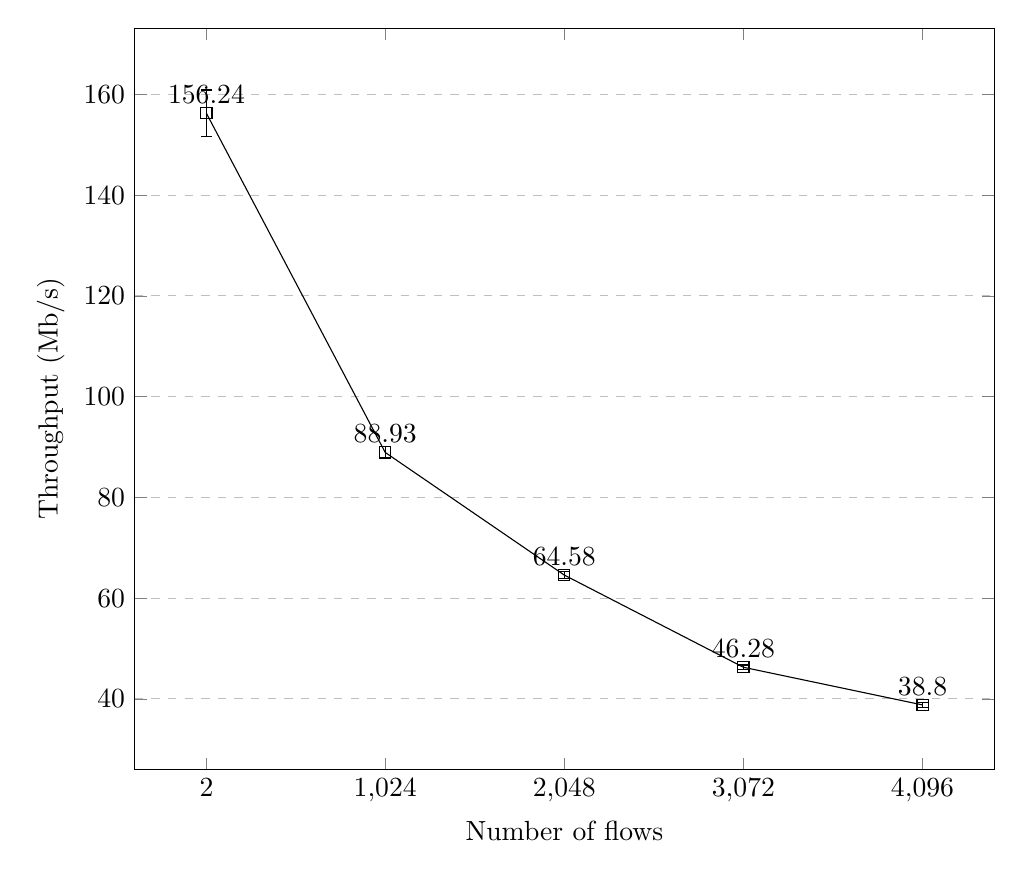
\begin{tikzpicture}
            \begin{axis}[
                xlabel={Number of flows},
                ylabel={Throughput (Mb/s)},
                ymajorgrids=true,
                grid style=dashed,
                ylabel near ticks,
                nodes near coords,
                scale only axis,       
                width=.9\textwidth,
                xlabel near ticks,
                xtick={2, 1024, 2048, 3072, 4096},
            ]
            \addplot[color=black, mark=square,error bars/.cd,y dir=both, y explicit]
            coordinates {
                (2, 156.24) +- (0.00, 4.64709)
                (1024, 88.93) +- (0.00, 1.20467)
                (2048, 64.58) +- (0.00, 0.65115)
                (3072, 46.28) +- (0.00, 0.4492)
                (4096, 38.8) +- (0.00, 0.52493)
            };
            \end{axis}
            \end{tikzpicture}
            \caption{Throughput per number of flows in one table}
            \label{graph:nflows}
        \end{subfigure}
         \hfill
        \begin{subfigure}[b]{.5\textwidth}
            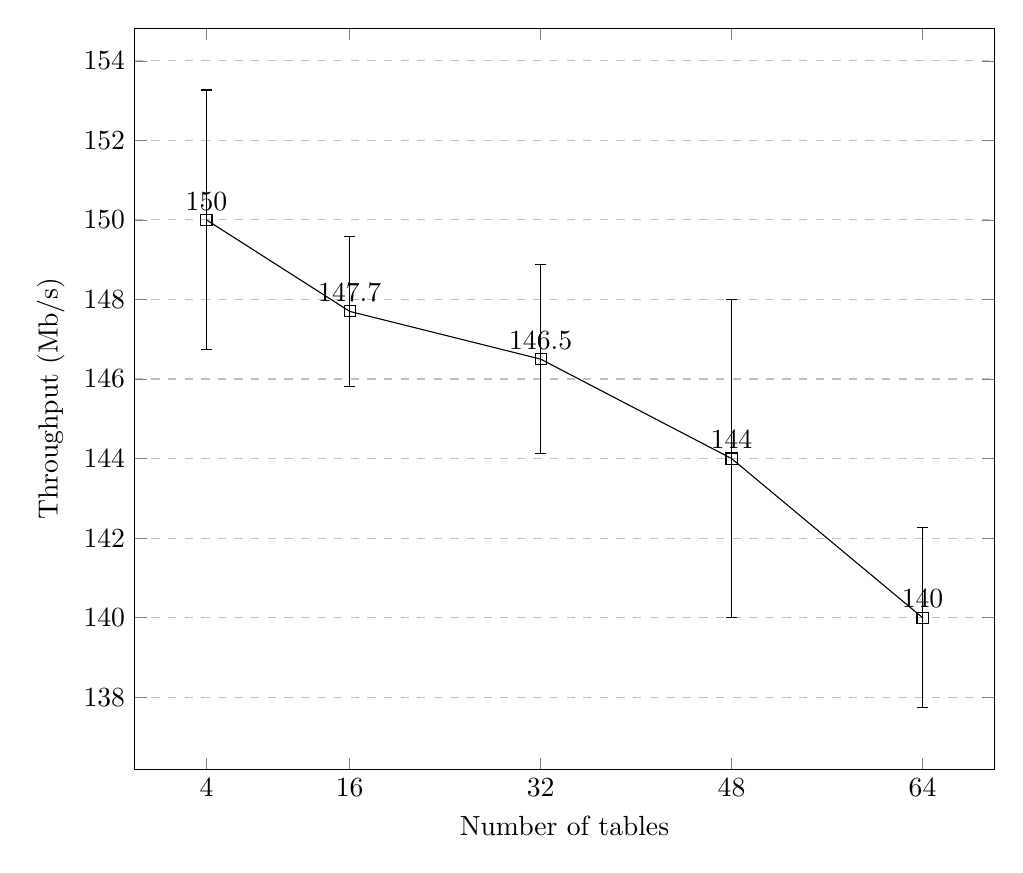
\begin{tikzpicture}
            \begin{axis}[
                xlabel={Number of tables},
                ylabel={Throughput (Mb/s)},
                ymajorgrids=true,
                grid style=dashed,
                ylabel near ticks,
                nodes near coords,
                scale only axis,       
                width=.9\textwidth,
                xlabel near ticks,
                xtick={4, 16, 48, 32, 64},
            ]
            \addplot[color=black, mark=square,error bars/.cd,y dir=both, y explicit]
            coordinates {
                (4, 150) +- (0.00, 3.26599)
                (16, 147.7) +- (0.00, 1.88856)
                (32, 146.5) +- (0.00, 2.36878)
                (48, 144)   +- (0.00, 4)
                (64, 140) +- (0.00, 2.26078)
            };
            \end{axis}
            \end{tikzpicture}
            \caption{Throughput per number of tables}
            \label{graph:ntables}
        \end{subfigure}
        \end{minipage}
            \caption{Influence of the number of installed flows on the throughput.}
            \label{graph:scaling}
        \end{figure}     
     
        The graphs in the Figure \ref{graph:scaling} shows that both cases have a strong influence over the switch performance. The most sensitive case is for one table shown in Figure \ref{graph:nflows}, as the number of flows increases the throughput decreases linearly. The increase in the number of tables, shown by the graph in the Figure \ref{graph:ntables}, also causes a linear decrease in the packet rate, though it is smaller than in the first case. These results were expected, since the software switch implements linear matching. Thus, this experiments were important to verify one improvement area for the software switch.     
     
    \subsection{Ping Round Trip Time}

    Round Trip Time (RTT) is the time between a data request and answer. Several factors might affect the total RTT and  influence network's latency. Two examples are: the number of nodes between two communicating hosts and the transmission medium. The time a packet takes to enter and leave a switch is also considered for the RTT. Thus, it is important to measure how much the software switch affects the RTT. 
    
    In order to measure the RTT between two hosts connected by our software switch - we also compare LINC and Trema -, the following steps are executed:
    
    \begin{enumerate}
    \item Creation of two Linux containers (LXC) - Host 1 and Host 2 - with a pair of virtual interfaces \textit{veth0} and \textit{veth1}. LXC is an operating system lightweight virtualization technology, in which it is possible to run multiple isolated Linux instances as containers. With LXC, we run two containers to serve as the network hosts.    
    \item Execution of a software switch instance with the container virtual ports attached to switch interfaces.
    \item Installation of two flows in the switch Flow Table to forward the traffic between the two hosts. 
    \item Configuration of Host 1 and Host 2 with IP addresses in the same network. In our test Host 1 is configured with the IP address 192.168.0.1 and host 2 as 192.168.0.2. 
    \item Execution of the \textit{ping} program in Host 1 to ping the address 192.168.0.2. Ping is a program to send and measure the time between an Internet Control Message Protocol (ICMP) "Echo request" and the ICMP "Echo Reply". The number of Echo requests sent is 100 and the packet sizes are 64Kb.
    \end{enumerate}

    Switch results comparison is shown in Table \ref{pingtable}. These tests give a good approximation for the software switch impact over the network delay, because it is connected directly to the hosts. As expected, because of the previous results, Trema is the most efficient among the userspace software switches. The ofsoftswitch13 obtains a low minimum RTT, with 0.304 ms, compared to the average of approximately 1ms. LINC has a very high RTT, with more than a half second to complete. This is not a surprise, because the throughput tests, shown in section \ref{sec:MaxBand}, revealed that LINC does not handle small packets efficiently.
    
    An acceptable RTT value depends on the application running over the network. Latency sensitive programs, like multiplayer online games, benefit from a low RTT. Considering a small network, with not many hops, the RTT in our software switch is acceptable.   

        % Please add the following required packages to your document preamble:
    % \usepackage{graphicx}
    \begin{table}[H]
    \caption{Ping Round Trip Time comparison between software switches}
    \label{pingtable}
    \resizebox{\textwidth}{!}{%
    \begin{tabular}{|l|c|l|c|c|}
    \hline
    \textbf{Software Switch} & \multicolumn{1}{l|}{\textbf{Minimum}} & \textbf{Average}           & \multicolumn{1}{l|}{\textbf{Maximum}} & \multicolumn{1}{l|}{\textbf{Standard Deviation}} \\ \hline
    ofsoftswitch13           & 0.30                                 & \multicolumn{1}{c|}{1.07} & 1.82                                 & 0.31                                            \\ \hline
    LINC                     & 303.90                               & \multicolumn{1}{c|}{554.77}                    & 821.48                               & 253.03                                          \\ \hline
    Trema                    & 0.12                                 & \multicolumn{1}{c|}{0.40} & 0.48                                 & 0.04                                            \\ \hline
    \end{tabular}
    }
    \end{table}

\section{Portability}

Software portability is the ability to compile and to run a program in different hardware architectures. For a network environment, more specifically OpenFlow, portability allows richer testbeds. Proposed as a friendly experimentation tool for multiple environments, the software switch implementation enables portability with few platform dependant modifications. Based on build scripts to install the OpenFlow 1.0 software switch on an OpenWRT \cite{OpenWrt} operating system image, \cite{yiakoumis2011}, we demonstrated portability building our OpenFlow 1.3 software switch for OpenWRT and running in a home wireless router.

The wireless router model for the software switch port is the TP-LINK TL-WR1043ND. This router already comes with a default OpenWRT image, however it is necessary to build a new image containing the software switch installed as an operational system package. 

\begin{itemize}
\item \textbf{Enhanced portability for different architectures}. Previously, the implementation considered only Intel based - i686 and x86_64, architectures. Byte order conversions were necessary because Intel processors byte-order are Little-endian, while the network follows the Big-endian order.  The MIPS processor of the wireless router model follows the same byte-order from the network. Standard Linux byte-order functions, from the library \textit{netinet/in.h}, do not check the system architecture but they do change the byte-order whatever the type of conversion called. For instance, if we call the function htons, to change the byte-order to network from host, and the value is already in the correct order, data is changed anyway. Thus, to avoid wrong values, we implemented byte-order conversions functions that check the system architecture before calling the standard procedures from \textit{netinet/in.h}.
\item \textbf{Netbee Remotion}. After the first execution, we realized the switch was consuming too much memory of the router limited ammount of RAM. From 32Mb of memory, the software switch was consuming 30Mb. After a memory profiling, we found that Netbee was the switch's most memory consuming component. While it is not a problem for a server or a machine with higher capacity, it is not true for a small embedded system like the wireless router. Therefore, we removed the Netbee library, reducing the average memory usage to less than 1Mb. Since the code is well structured, the new parsing implementation was trivial. Only a simple redefinition of the parsing function in the packet handler interface was necessary. This situation also demonstrated the code's friendliness. 

\end{itemize}

The implementation of an OpenFlow 1.3 switch for a wireless router opens a myriad of opportunities in the area of Software Defined Wireless Networking. Experimenters might take advantage of the new features implemented by our software switch. Flow metering, for example, is a simple yet powerful mechanism to provide bandwidth control in home environments. Also, creation of firewall blocking rules is made easy by OpenFlow, since field matching is a natural  operation for an OpenFlow switch.

\chapter{Conclusion}
\label{cap:conclusion}

Six years ago SDN and OpenFlow caused a stir in the world of computer networks. Although data and control plane separation is not a new idea, the flexibility and programmability enabled by OpenFlow started a wave of industry efforts to support the protocol in their products. Several OpenFlow 1.0 switches, controllers and test frameworks emerged from this movement, confirming the growing interest in this technology. Large networks operators, such as Google and Facebook, embraced OpenFlow interested in its potential. An organization, named Open Network Foundation, was created to speed up the OpenFlow development and adoption. Quickly, new versions of the protocol were released. This time, however, implementations did not arouse at the same time.

To keep up with the pace of the technology and to enable research capable of leveraging the new functionalities, we found the need to implement an OpenFlow 1.3 software switch. More than a full compliant implementation, requirements included minimal performance and ease of experimentation. This effort lead to the open source software implementation of the first OpenFlow 1.3 switch. 

Today, the software switch is a well known open source project and a cheap and friendly option to experiment OpenFlow 1.3. Although new software switches supporting OpenFlow 1.3 are now available, this work is still a solid and relevant option to prototype and develop new OpenFlow applications. In the next two sections, we present some significant obtained results and notorious use cases. Finally, we conclude this chapter discussing future areas for research and improvement in the software switch.     

\section{Results}
\label{sec:results}

In this section we list positive results achieved on the dissemination of our work:  

\begin{itemize}
\item \textbf{Development of an Open source community.} The choice of using GitHub to host the code proved to be a great way to reach a high number of users. Figure \ref{fig:ghstats}, shows information confirming the tool's popularity. In a 14 days interval, the software switch repository had 3125 accesses, with 796 unique visitors and cloned 97 times. 

When it comes to code contributions, there are 15 users listed in GitHub that submitted pull requests. Also, there is a number of contributors that send patches through other means.

This result is very important because the creation of a community around open source code gives it visibility, helps to spread the software and speed up reports of detected bugs. 

\begin{figure}[H]
\centering
\includegraphics[height=20cm,width=\textwidth,keepaspectratio]{eps/GH.pdf}
\caption{GitHub statistics.}
\label{fig:ghstats}
\end{figure}

\item \textbf{Part of Mininet installation options.} The software switch is included among the installation options of Mininet. It makes easier for users to start experimenting with OpenFlow 1.3. Another great effect is the numbers of users reached, since this work is the default OpenFlow 1.3 userspace switch in Mininet.      

\item \textbf{Publications.} This work gave origin to three publications. The first paper is about IPv6 support on OpenFlow. The second is an invited paper bringing perspectives on SDN for home network. These ideas were inspired by the software switch port to OpenWRT. Finally, the last paper is an overall presentation of this project, highlighting architectural and implementation details. These publications are listed on Annex \ref{AnnexB}.  
\end{itemize}


\section{Use Cases}
\label{sec:cases}

Known use cases show that the software is an important tool in the advance of the state of art on SDN research and development. As there is a large number of projects that are using or have made use of our work, we will list some notorious examples: 

\begin{itemize}
\item \textbf{Base for new OpenFlow features implementation.} The ONF group responsible by the addition of new OpenFlow features decided to publish new features only if properly implemented and tested. As OpenFlow 1.3 basic functionalities is required for 1.4 and 1.5, the Extensions Work Group chose our work as one of the software switches as a base to prototype new functionalities \cite{ONFproto}. 

\item \textbf{Academic.} The software switch has found good adoption by the academic community. For instance, works published in renowned conferences \cite{Reitblatt:2013:FDF:2491185.2491187} \cite{Bianchi:2014:OPP:2602204.2602211} and master dissertations \cite{Paris} \cite{ShahmirShourmasti656472} cite our software as the OpenFlow 1.3 switch chosen for their experiments.  

\item \textbf{Industry.} Industrial development is harder to track because it is usually closed. However, one successful case is in the development of an application for the Open Network Operating System (ONOS). Built by two companies' teams, Dell and ON.Lab, the Segment Routing implementation used the software switch for its simplicity \cite{ONOS}.         
\end{itemize}

\section{Future Work}

Each architectural component from the software switch has space for improvements. New algorithms and data structures are objects of study for the Flow Table matching. More complex and precise algorithms for rate limiting might be considered for better Meter Table performance. As for groups, new bucket select types may be a subject for academic research. 

While there are open ideas for further research and development, some optimizations and features are planned for the software switch in the medium-term. These major improvements are listed below:

\begin{itemize}

\item \textbf{Support for OpenFlow 1.4 and 1.5}. OpenFlow 1.4 and 1.5 are extensions of OpenFlow 1.3 and it would be good to keep the pace with the OpenFlow evolution. Some OpenFlow 1.4 and 1.5 features are already implemented, as stated in section \ref{sec:cases}. However, we would like to have both versions supported in one single switch running instance, without need to split the code in two different programs.

\item \textbf{Hash based match.} Results found in experiments presented on section \ref{sec:bandflows} show a huge loss in performance due to linear matching. To solve this problem, flows entries might be represented as hash value into the Flow Table. Then, packet fields could also be turned into a hash and looked up in the Flow Table. This would give constant performance for the Flow Table look up. However, some relevant questions arise: 

    \begin{itemize}
    \item How to handle flow priority? Since flows should be matched in order of priority, how to ensure the first hash value for a flow is the one with higher priority? 
    \item How to deal with field masking? Some flow match fields may have a mask, so they should be considered in the hash calculation. The question is how to efficiently search and apply these masks to the packet hash calculation. 
    \end{itemize}

The search for an answer for these questions opens space for new research in OpenFlow and SDN, since these questions are not only related to the software switch. 
  
\item \textbf{New packet parsing engine}. The software switch relies on Netbee library to parse packets. While Netbee adds flexibility and extensibility for the parsing and the ease of addition of new protocols to OpenFlow, its code is neither frequently updated, nor following dependencies upgrades. This breaks the software switch compilation in more recent Linux versions, because of more recent versions of libraries required by Netbee. Due to the number of compilation issues related to Netbee, a new packet parsing module must replace the current third party library.

\end{itemize}


% --- Finaliza a parte no bookmark do PDF, para que se inicie o bookmark na raiz ---
\bookmarksetup{startatroot}%
% ---


% ---- ELEMENTOS P\'{O}S-TEXTUAIS ----
\postextual

% ---- Refer\^{e}ncias bibliogr\'{a}ficas ----
\bibliography{tese}

% ---- Ap\^{e}ndices ----

% ---
% Inicia os ap\^{e}ndices
% ---
%\begin{apendicesenv}
%
%% Imprime uma p\'{a}gina indicando o in\'{\i}cio dos ap\^{e}ndices
%\partapendices
%
%%  ----------------------------------------------------------
% ---- Anexos ----

% ---
% Inicia os anexos - opcional
% ---
\begin{anexosenv}

% Imprime uma p\'{a}gina indicando o in\'{\i}cio dos anexos
\partanexos

\chapter{P4 code of BNG}
\label{annex:p4code}


% ---
\chapter{Publications}
% ---
\label{AnnexB}
Three papers were published during this work and are listed below. 

\begin{itemize}

\item Juan Sebastian Mejia Vallejo , Christian Esteve Rothenberg. "Broadband Network Gateway implementation using a programmable data plane processor". In  X DCA/FEEC/University of Campinas (UNICAMP) Workshop (EADCA),  Campinas, Brazil, October 26-27, 2017

\item Juan Sebastian Mejia, Christian Esteve Rothenberg. "Network Address Translation using a Programmable Dataplane Processor". In 7º Workshop em Desempenho de Sistemas Computacionais e de Comunicação (Wperformance) XXVIII Congresso da Sociedade Brasileira de Computação - CSBC 2018, Natal, 22 to 26 of Jule, 2018.

  
\end{itemize}



% ---- INDICE REMISSIVO ----

\printindex

\end{document} 